\chapter{Testování softwaru}
%SMAZAT!!
%Testování aplikací je nedílnou součástí jejich vývoje a~v~dnešní době se tomuto oddílu tvorby aplikací věnuje čím dál více pozornosti. Dá se rozdělit do různých skupin, např. podle toho, kdy se testování provádí, jakým způsobem se provádí, jak se k~testované aplikaci přistupuje, či jaká část aplikace se podrobuje testům.

%Jednou z~důležitých součástí je testování grafického uživatelského rozhraní. Zde se testeři soustředí na to, zda daná aplikace vypadá tak, jak to požadují vývojáři a~návrh, a~zda grafické prvky správně fungují. Dále se zaměřuje na to, zda je aplikace přívětivá k~uživateli a~práce s~ní není příliš komplikovaná.

%Při testování grafického uživatelského rozhraní se může spousta testů mnohokrát opakovat, a~proto je snaha tyto testy nějak automatizovat. K~tomu se může využít některý z~nástrojů k~tomu určený. Cílem této práce je seznámit se s~některými z~těchto nástrojů, jeden z~nich vybrat a~pomocí něj vytvořit sadu ukázkových testů svou filosofií zapadajících do předmětu KIV/OKS.

Na začátek je potřeba vysvětlit některé pojmy z~oblasti testování. Budeme vycházet hlavně z~\citep{RizeniKvalitySW} a~\citep{Patton}.

	\section{Požadavky}
	Požadavky zachycují přání zákazníka na funkcionalitu softwaru. Dělí se na dvě skupiny:
		\begin{itemize}
			\item Funkční -- popisují funkčnost služby vykonávané systémem, tedy co má vykonávat. Patří sem např.:
				\begin{itemize}
					\item Uživatel bude moci vytvořit záznam pro nového zákazníka.
					\item Systém automaticky odhlásí uživatele po 3 minutách nečinnosti.
				\end{itemize}
			\item Mimofunkční -- popisují určité vlastnosti systému, či omezující podmínky. V~podstatě říkají, jaký by systém měl být. Sem patří např.:
				\begin{itemize}
					\item Modul "Správa klientů" bude dostupný pouze uživatelům s~rolí správce.
					\item Systém bude použitelný při zátěži 1000 uživatelů.
				\end{itemize}
		\end{itemize}
	
	Je vhodné, aby se testeři zabývali i~požadavky, neboť mohou již v~rané fázi vývoje zachytit ty chybně formulované (nekonzistentní, neproveditelné, nekompletní, netestovatelné, nejednoznačné, více požadavků zapsaných jako jeden apod.).
	
	\section{Specifikace požadavků na software}
	Funkční i~mimofunkční požadavky zákazníka, jejich analýza a~dokumentace a~všeobecný popis systému se zapisuje do dokumentu nazvaného specifikace požadavků na software. Na základě tohoto dokumentu probíhají následující fáze vývoje, proto je jeho správnost velmi podstatná.
	
	K~tomuto dokumentu se poté vztahuje i~testování, konkrétně funkční testování, které kontroluje, zda software vyhovuje a~splňuje požadavky zákazníka.
	
	\section{Kvalita softwaru}
	Kvalita softwaru je velmi obtížně definovatelný pojem. Pro její definici vzniklo několik norem. Ty jsou dnes zastaralé či nekonzistentní, proto jsou nahrazovány jednotným systémem norem ISO/IEC 25000-25099 v~rámci projektu SQuaRe (Software Quality Requirements and Evaluation).
	
	Např. norma ISO/IEC 25010 říká, že kvalita softwaru je míra, do jaké softwarový produkt splňuje stanovené a~implicitní potřeby, je-li používán za stanovených podmínek.
	
		\subsection{FURPS}
		Dnes nejčastějším modelem kvality softwaru je tzv. FURPS, který vytvořila společnost Hewlett-Packard. Ten kvalitu popisuje pomocí těchto pěti charakteristik:
			\begin{itemize}
				\item Functionality (Funkčnost) -- soubor požadované funkcionality, schopností a~bezpečnostních aspektů systému.
				\item Usability (Použitelnost) -- snadnost použití, konzistence, estetika, dokumentace apod.
				\item Reliability (Spolehlivost) -- četnost a~závažnost selhání, doba bezporuchového běhu, správnost výstupů, zotavení atd.
				\item Performance (Výkonnost) -- odezva systému, výkon za různých podmínek, požadavky na systémové prostředí.
				\item Supportability (rozšiřitelnost/podporovatelnost) -- škálovatelnost, udržovatelnost, testovatelnost, snadnost konfigurace.
			\end{itemize}
		Většinou se setkáme s~modelem FURPS+, který navíc přidává kategorie jako omezení návrhu, požadavky na implementaci, požadavky na rozhraní a~požadavky na fyzické vlastnosti.
			
	\section{Chyba, defekt, selhání}
	Během vývoje softwaru se do dokumentů či zdrojových kódů dostávají defekty, způsobující chyby a~selhání. Tyto pojmy je velmi důležité rozlišovat. V~následujících odstavcích bude jejich význam vysvětlen.
	
	Selhání nastává v~případě, že jeden nebo více výstupních stavů aplikace se odlišuje od stavu správného (nesplňuje specifikaci, případně specifikace nebyla kompletní nebo jednoznačná).
	
	Právě toto odchýlení od očekávaného stavu se nazývá chybou. Původ chyby se nazývá defekt a~označuje se tak vada v~kódu či datech. Nejčastěji jej způsobí programátor chybou v~kódu, špatným návrhem, nedostatečně či nesprávně pochopenou specifikací, nebo záměrnou sabotáží.
	
	Jednotlivé pojmy na sebe tedy navazují následovně (viz obrázek \ref{Bug}): defekt (aktivace) $\to$ chyba (šíření) $\to$ selhání (příčina)\dots
	\begin{figure}[ht!]
		\centering
		\caption{Šíření chyby mezi systémy. Selhání systému A~je pro příjemce jeho služby (systém B) externím defektem, který může vést k~chybě a~ta poté opět  k~selhání. Zdroj \citep{RizeniKvalitySW}}
		\label{Bug}
		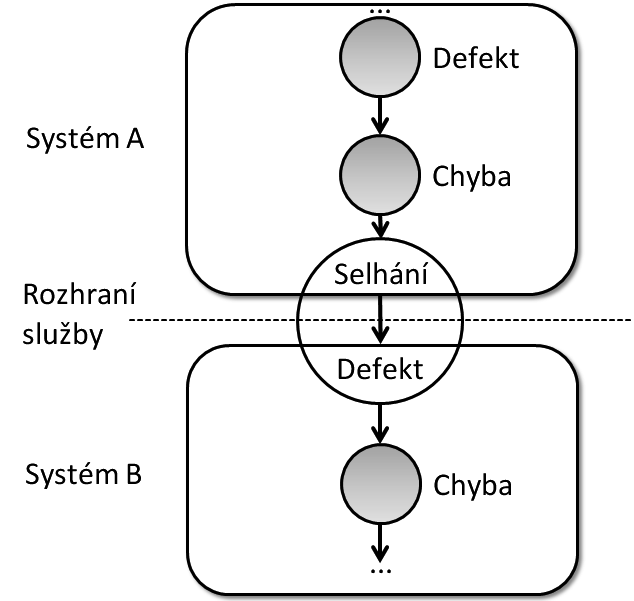
\includegraphics[width=8cm]{img/Bug.png}
	\end{figure}
	
	\section{Testování softwaru}
	Definice pojmu testování softwaru se více či méně liší téměř v~každé publikaci. V~knize \citep{RizeniKvalitySW} je testování definováno jako proces řízeného spouštění softwarového produktu s cílem zjistit, zda splňuje specifikované či implicitní potřeby uživatelů. Je zde důležité slovo spouštění, které z~testování vyřazuje metody statické analýzy. Obecněji se však i~tyto metody do testovaní řadí a~jejich použití bývá ve vývoji softwaru vhodné.
	
	Záměrem testování již není nalézat defekty, jak tomu bylo dříve. Nyní je jím získat informaci o~kvalitě softwaru a~o~tom, jak moc splňuje požadavky zákazníka.
	
	\citep{Patton} uvádí řadu axiomů (obecně přijímaných pravd, které se nemusejí dokazovat) o~testování. Čtyři nejdůležitější z~nich jsou:
		\begin{itemize}
			\item Žádný program není možné otestovat kompletně -- počet vstupů, výstupů a cest, které vedou skrze software je příliš velký.
			\item Testování softwaru je postavené na riziku -- nemožnost otestování všech případů vede k~tomu, že je možné nezachytit defekt ve scénáři, který se netestoval. Je proto důležité správně odhadnout možná rizika a~testováním je minimalizovat.
			\item Testování nikdy nemůže prokázat, že chyby neexistují -- testováním pouze můžeme dokázat, že chyby existují, ale jelikož není možné software kompletně otestovat, existenci chyb vyloučit nelze.
			\item Čím více chyb najdeme, tím více jich v~softwaru je -- kvůli tomu, že programátoři mívají špatné dny nebo dělají často stejné chyby, se chyby vyskytují ve skupinách. To znamená, že objevení jedné chyby zvyšuje pravděpodobnost dalších takových podobných chyb.
		\end{itemize}
		
		\section{Úrovně testování}
		Během vývoje softwaru se testování nechá rozdělit do různých skupin, např. podle toho, kdy se testování provádí, jakým způsobem se provádí, jak se k~testované aplikaci přistupuje, či jaká část aplikace se podrobuje testům. Rozlišují se např. tyto čtyři fáze:
			\begin{itemize}
				\item Testování jednotek (Unit Testing) -- testování provádí obvykle sám programátor, který se snaží prokázat správnost fungování jednotlivých jednotek (nejmenších testovatelných součástí aplikace).
				\item Integrační testování (Integration Testing) -- testuje se zapojení výše uvedených jednotek do aplikace. Správná funkčnost jednotek nezaručuje správnou funkčnost výsledné aplikace.
				\item Systémové testování (System Testing) -- testuje se, zda aplikace splňuje požadavky zákazníka. Patří sem nejen funkční testování, ale i~mimofunkční.
				\item Akceptační testování (User Acceptance Testing, UAT) -- zde provádí testování sám zákazník a~neomezuje se pouze na testování jako takové, ale na splnění před dohodnutých kritérii (dokumentace, manuály apod.).
			\end{itemize}
			
		\section{Testování grafického uživatelského rozhraní}
		